\chapter{Event Selection and Reconstruction}
\section{Data Sample}
In this analysis, we use the full data which was collected by the Belle detector at the KEKB asymmetric-energy $e^+e^-$ colider\
(with one side is 3.5 GeV and another is 8GeV).The data on the $\Upsilon(4S)$ resonance is used, with the integrated luminosity is 710 $fb^-1$.\
The total number of $B\bar{B}$ event from experiment 7 to 65 is $771.581\pm10.566$ million. 
\subsection{Monte Carlo sample}
And there are various officially produced Monte Carlo have been used in the analysis, There are generic, continuum and rare MC. \
The generic Monte Carlo is about the decay of B mesons where b quark decay into a c quack, and the sample include two kinds, one is called "charged", which refer to the decay of\
 $\Upsilon(4s)$ into $B^+ B^-$ pairs, the other is called "mixed", which refer to the decay of $\Upsilon(4s)$ into $B^0 \bar{B^0}$ pairs.There are ten streams of generic MC available totally\
corresponding to ten times of Belle I data size.In this study, six stream of generic MC are used for now.Another kind of MC sample is the continuum, where the events have no $\Upsilon(4s)$ been\
produced, and the corresponding processes are $e^+ e^-$ pair decay to $u, d, s, c$ quark pairs, There are six streams of continuum MC available totally. All six streams of the continuum MC sample\
are used in this study.The other is rare MC sample which cover all the non $b \rightarrow c$ B decay transitions. The rare MC sample contain the 50 times the data luminosity\
for $b \rightarrow u \ell \nu$ transition, and 20 times data size for all other non $b \rightarrow c$ channel.\\
For signal decay study, all signal sample with $B \rightarrow K^{(*)} \nu \bar{\nu}$ which $K^{(*)}$ is stand for are generated with EvtGen package, and detector simulation is done with GEANT package.\
In the decay generated process, model VSS is used to simulate $\Upsilon(4s)$ decay $B^+ B^-$ and model VSS\_BMIX dm is used to simulate $\Upsilon(4s)$ decay $B^0 \bar{B^0}$ with $B^0 \bar{B^0}$\
mix condition turn on.The $B \rightarrow K^{(*)} \nu \bar{\nu}$ for all $K$ channel are used phase space decay model to describe.There are 771,0000 signal MC sample used for each $K{(*)}$ channels.\
%\subsection{Blind Analysis}
\section{Event Selection}
In this study, we only consider events passed through both HadronB(J) skim and full reconstruction skim.
Candidate $e^+ e^- \rightarrow \Upsilon(4s) \rightarrow B B $ events are characterized by a fully reconstructed tag-side \
B meson. The remaining particles are assumed to be products of signal-side B meson.
\subsection{Hadronic Tag}
In order to study the mode which include missing particle, e.g., neutrinos, We reconstruct the hadronic B meson, which called $B_{tag}$ by using the Fullrecon package in Belle library.The latest version Fullrecon package with the Neurobayes neural networks\cite{ref:Feindt2011} have the better performance on the candidate selection, and also increase the purity and efficiency that compare to the old Fullrecon package. \
The $B_{tag}$ candidates can reconstructed in one of the following mode:\\
$B^0 \rightarrow D^{(*)-} \pi^+ $ , $ D^{(*)-} \rho^+$ , $ D^{(*)-}a^+_1$ , $ D^{(*)-} D^{(*)+}_s$ ,etc.\\
$B^+ \rightarrow\bar{D}^{(*)0} \pi^+$ , $ \bar{D}^{(*)0} \rho^+$ , $ \bar{D}^{(*)0}a^+_1$ , $ \bar{D}^{(*)0} D^{(*)+}_s$ ,etc.\\
$D$ meson can reconstructed by:\\
$D^- \rightarrow K^0_s \pi^- \pi^0$ , $K^0_s \pi^- \pi^+ \pi^-$ , $K^+ \pi^+ \pi^-$ , $K^+  \pi^- \pi^-\pi^0$ ,etc. \\
\vspace*{1mm}
$\bar{D^0} \rightarrow K^+ \pi^-$ , $K^+ \pi^- \pi^0$ , $K^+ \pi^- \pi^+ \pi^-$ , $K^0_s \pi^0$ , $K^0_s \pi^- \pi^+$ , $K^0_s \pi^- \pi^+ \pi^0$ , $K^- K^+$ ,etc. \\
\vspace*{1mm}
$D^{*-}(D^*0) \rightarrow \bar{D^0} \pi^-(\bar{D^0} \pi^0$ , $ \bar{D^0} \gamma)$ ; $D^{*+}_s \rightarrow D^+_s \gamma$ ; $D^+_s \rightarrow K^0_s K^+$ and $K^+ K^- \pi^+$ .\\
\vspace*{2mm}
There are totally 1104 hadronic decay channels include. \
For the $B_{tag}$ candidate selection, choose the best candidate by using the event-wide rank according to NeuroBayes output with continuum suppression(cont\_NBRank).We also reject events with wrong sign reconstruction best $B_{tag}$\
will be rejected. i.e., reject the event of the signal side $B^+ \rightarrow K^+ \nu \bar{\nu}$ with the best $B_{tag}$ candidate $B^0$.  

\subsection{Particle Selection Criterion}
\begin{itemize}[leftmargin=*]
\item \textbf{Track Selection}\\
The track particles are all collected from MDST\_CHARGED bank after forming a $B_{tag}$, we require the transverse momentum $p_t$ greater than 0.1 GeV/c, and also require the impact parameter in radial direction\
$|dr| <$ 2cm, and in beam direction $|dz| <$ 5cm.
\item \textbf{Charge Particle Identification}\\
\textbf{$\bm{K^\pm}$ candidates} of the particle identification likelihood ratio $\mathcal{L}_{ K \pi}$ > 0.6,  $\mathcal{L_{\mu}}$ < 0.9\\
and  $\mathcal{L}_{e}$ < 0.9. \\
\textbf{$\bm{\pi^\pm}$ candidates} of the particle identification likelihood ratio $\mathcal{L_{ K \pi}}$ < 0.4,  $\mathcal{L_{\mu}}$ < 0.9\\
and  $\mathcal{L}_{e}$ < 0.9.\\
\textbf{$\bm{e^\pm}$ candidates} of the particle identification likelihood ratio $\mathcal{L}_{e}$ > 0.9, and also require \\
$\mathcal{L_{\mu}}$ < 0.9.\\
\textbf{$\bm{\mu^\pm}$ candidates} of the particle identification likelihood ratio $\mathcal{L_{\mu}}$ < 0.9.
\item \textbf{$\bm{K_s}$ candidates selection}\\
The $K_s$ candidates are all collected from MDST\_Vee2 bank, require \\ 
goodks == 1, $m_{Ks} > 0.4826$ and $m_{Ks} < 0.5526$ and also the $\chi ^2$ given by Vee2 bank must < 100.
\item \textbf{$\bm{\pi^0}$ candidates selection}\\ 
the $\pi0$ candidates are collected from MDST\_pi0 bank, $\pi^0$ are reconstructed by two photon candidates with an energy of 50MeV at least, \
The invariant mass of the photon pair should be within 117.8$MeV/c^2$ and 150.2$MeV/c^2$.

%and asymmetry $\alpha = \frac{|E_{\gamma1}−E_{\gamma2} |}{|E_{\gamma1}+E_{\gamma2} |}$ is smaller than 0.9.

\item \textbf{$\bm{K_L}$ candidates selection}\\
Collected from MDST\_klong, the $K_L$ candidates have to survive more than two KLM layers.
\item \textbf{$\bm{K^{*\pm}}$ candidates} are reconstructed in two different mode, there are $K^{*\pm} \rightarrow K^\pm \pi^0$ and $K^{*\pm} \rightarrow K_s \pi^\pm$. \
The $K^{*\pm}$ mass have to within the window, 0.8166 < $m_{K^*}$ < 0.9666. , and $K^{*0}$ mass have to within the window, 0.8166 < $m_{K^*}$ < 0.9666.
\item \textbf{$\bm{K^{*0}}$ candidates} are reconstructed in a charge K and a $\pi$. Their invariance mass must within the window 0.8211 < $m_{K^*}$ < 0.9711. \
The invariance mass distribution of
$K^{*0}$, $K^{*\pm}\rightarrow K^\pm \pi^0 $ and $K^{*\pm} \rightarrow K_s \pi^\pm$ are shown in Fig. \ref{K0mass}, \ref{kpi0mass} and \ref{kspimass} respectively.
\end{itemize}

\begin{figure}[h]
	\centering
	\subfigure[$K^{*0}$ mass.]{
		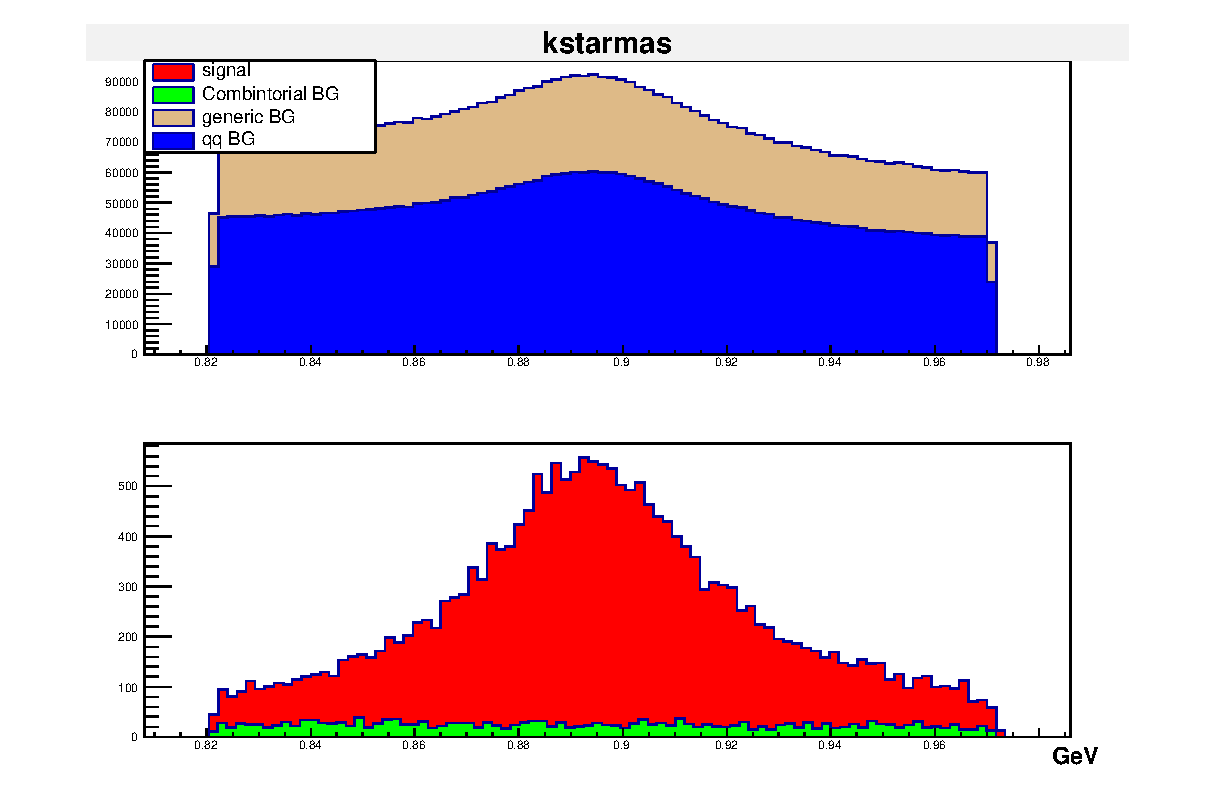
\includegraphics[width=0.45\textwidth]{eventselection_figure/kstarmas_1025_1_b0kst.eps}
		\label{K0mass}
	}
	\subfigure[$K^{*\pm} \rightarrow K^\pm \pi^0$ mass.]{
		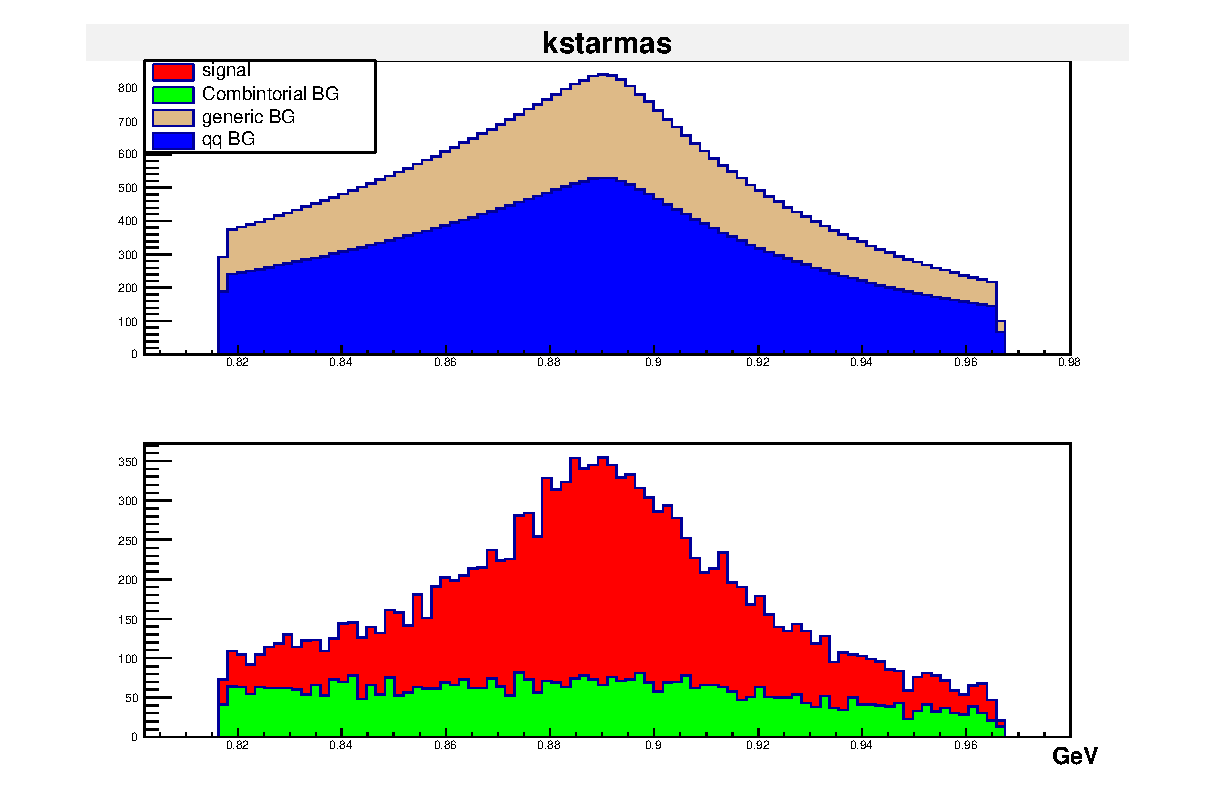
\includegraphics[width=0.45\textwidth]{eventselection_figure/kstarmas_1025_1_kpi0.eps}
		\label{kpi0mass}
	}
	\subfigure[$K^{*\pm} \rightarrow K_s \pi^\pm$ mass.]{
		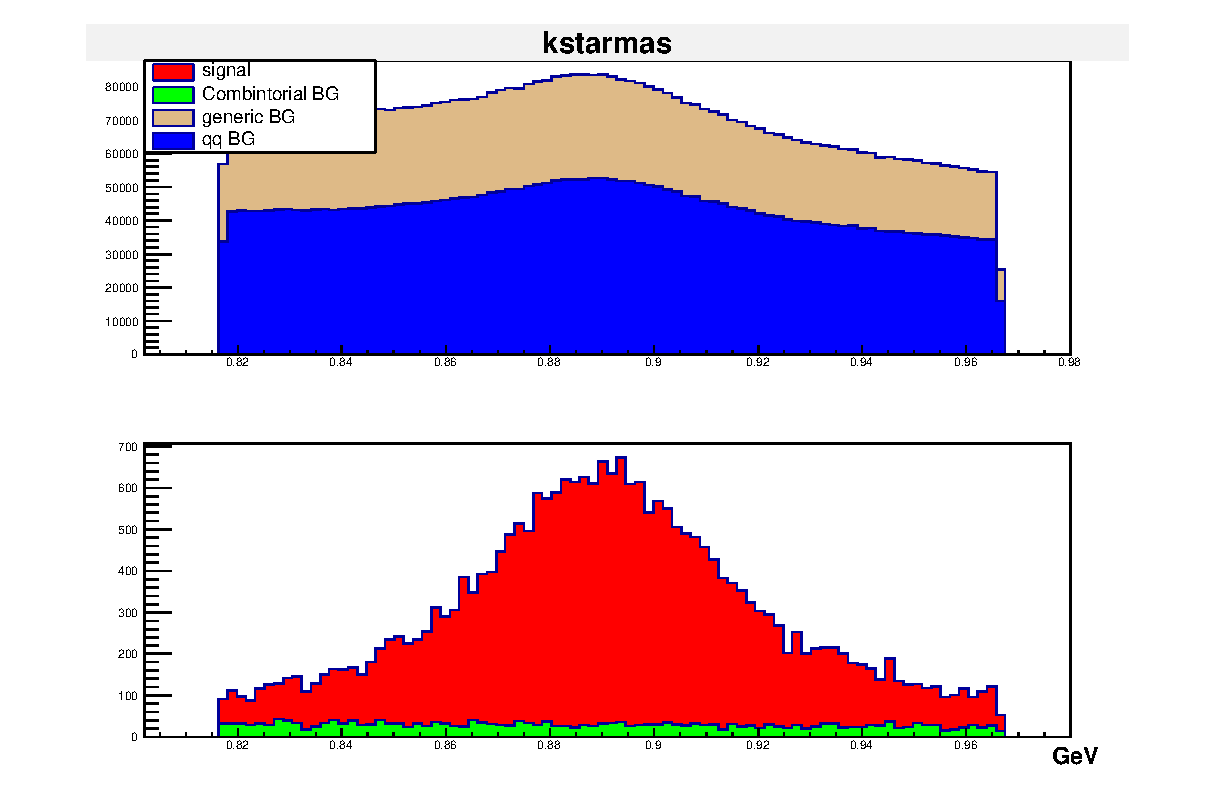
\includegraphics[width=0.45\textwidth]{eventselection_figure/kstarmas_1025_1_kspi.eps}
		\label{kspimass}
	}
	\label{kstarmass}	
	\caption{$K^*$ mass, red represent signal, green represent the combinatorial background,  brown represent the generic background and blue represent continuum background.}
\end{figure}

\subsection{Basic Selection}
It is necessary to apply the basic selection to get rid of the obvious background before we do the Neural-Network bases analysis. This pre-cut can improve the efficiency of \
training result.
\begin{itemize}[leftmargin=*]
\item \textbf{$\bm{B_{tag}}$ selection}\\
The $B_{tag}$ candidates are require to match $M_{bc}$ > 5.24 GeV/$c^2$ and $|\Delta E|$ < 0.05 GeV, the loose requirement on tag side $M_{bc}$ and $|\Delta E|$. \
We also require the $\bm{O_{tag}}$ with continuum suppression, we make a lower cut on log($o_{tag}$) > -7. The distribution of tag-side $M_{bc}$, $|\Delta E|$ and $O_{tag}$ are shown in Fig. \ref{fig:tagbmbc}, \ref{fig:tagbde} and \ref{fig:nbout} respectively.
\item $\bm{E_{ecl}}$\\
$E_{ecl}$ is the total remaining energies of the cluster in ECL detector which are not associated with $B_{tag}$ daughter particle and signal visible candidate.We make the different thresholds on different part of ECL, there are:
\begin{itemize}[leftmargin=*]
\item $E_{cluster}$ > 0.05GeV on barrel.
\item $E_{cluster}$ > 0.10GeV on forward end-cap.
\item $E_{cluster}$ > 0.15GeV on backward end-cap.
\end{itemize}
We define that $E_{ecl}$ < 0.3 GeV as the signal region, $E_{ecl}$ > 0.45 GeV as the sideband region, and set the upper cut on $E_{ecl}$ < 2 GeV.The $E_{ECL}$ distribution are shown in Fig. \ref{fig:sumecl}.
\item \textbf{Veto}\\
We expect there are nothing left beside the $B_{tag}$ and signal-side $B_{sig}$ candidate, we veto the events which have the additional track and also require there are no \
$K_L$ candidates left. We do not require the $\pi^0$ veto, because it'll drop too much signal efficiency. Instead make a $\pi^0$ veto, we make it as the training variable for NeuroBayes.\\
The efficiency table for each mode is shown in table \ref{t:efficiency_k} to \ref{t:efficiency_ks}.
\end{itemize}
\begin{figure}[ht]
	\centering
	\subfigure[$K^{\pm}$ mode.]{
		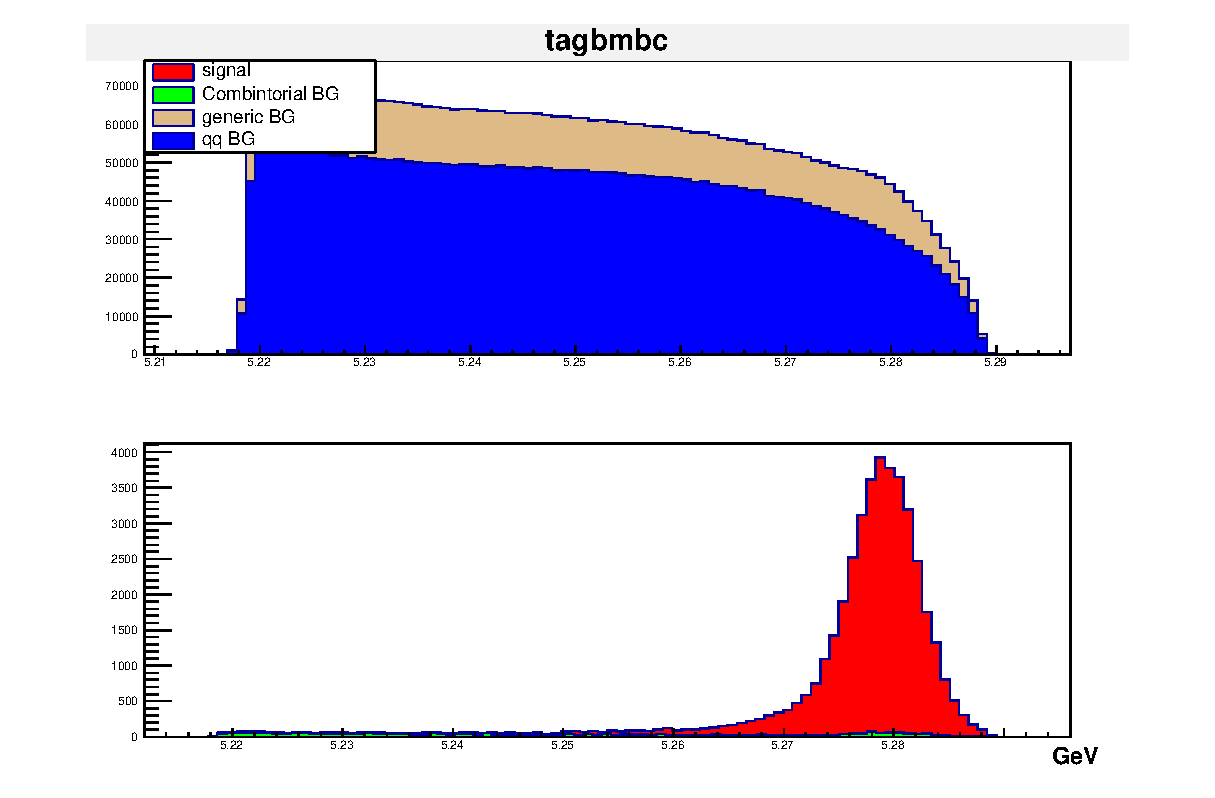
\includegraphics[width=0.45\textwidth]{eventselection_figure/tagbmbc_1025_1.eps}
		\label{kmbc}
	}
	\subfigure[$K^{*\pm} \rightarrow K^\pm \pi^0$ mode.]{
		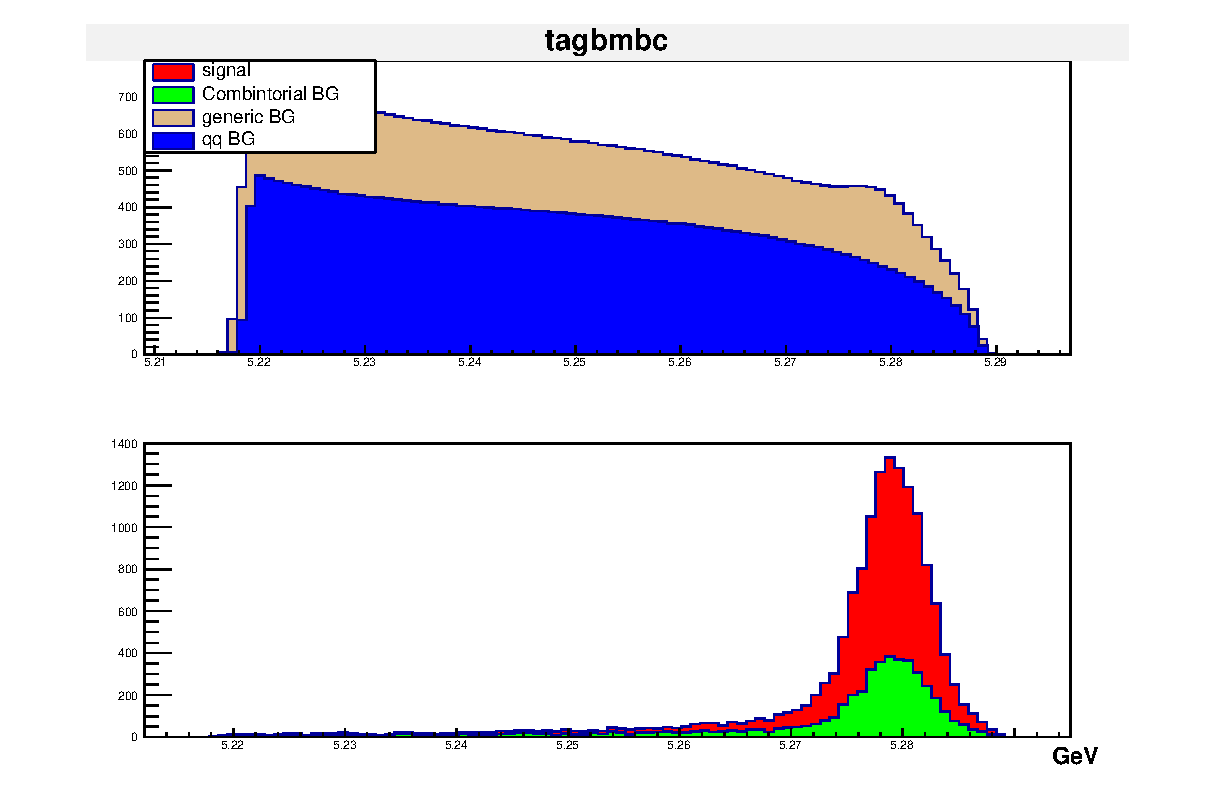
\includegraphics[width=0.45\textwidth]{eventselection_figure/tagbmbc_1025_1_kpi0.eps}
		\label{kpi0mbc}
	}
	\subfigure[$K^{*\pm} \rightarrow K_s \pi^\pm$ mode.]{
		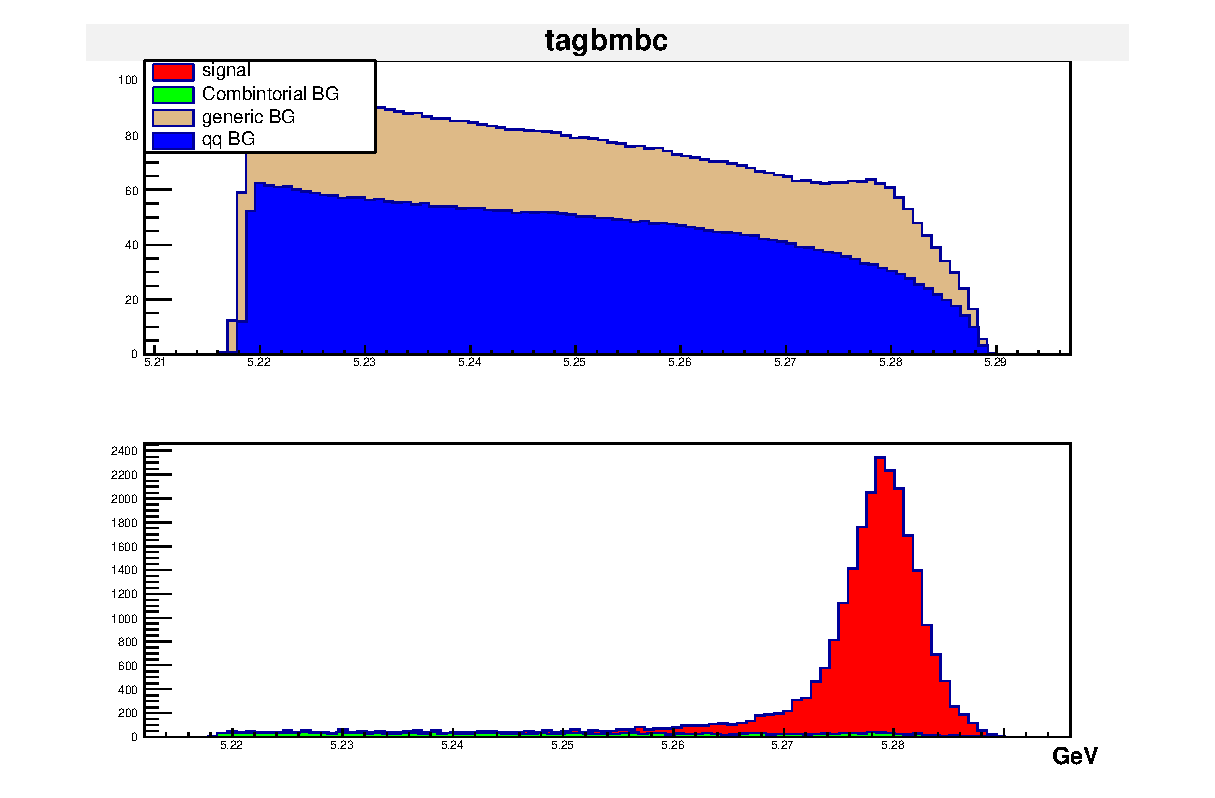
\includegraphics[width=0.45\textwidth]{eventselection_figure/tagbmbc_1025_1_kspi.eps}
		\label{kspimbc}
	}
    \subfigure[$K^{*0}$ mode.]{
		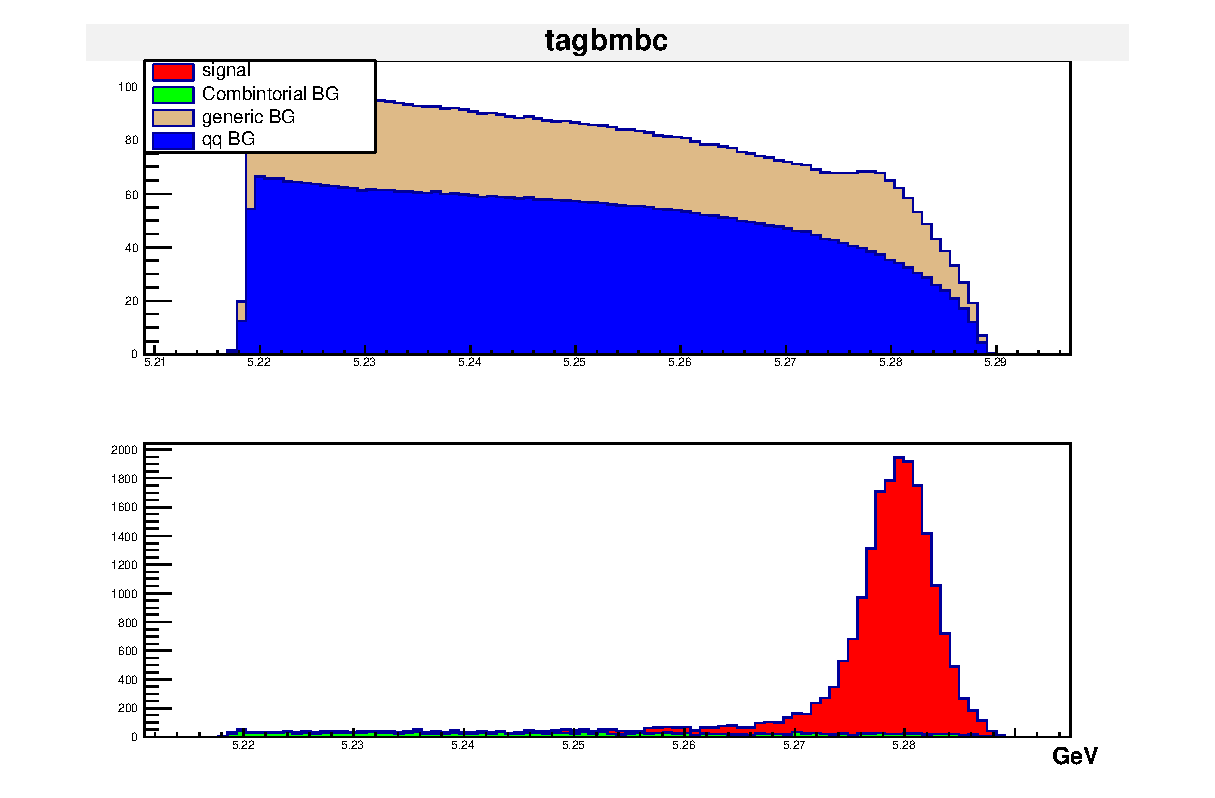
\includegraphics[width=0.45\textwidth]{eventselection_figure/tagbmbc_1025_1_b0kst.eps}
		\label{k0mbc}
	}
    \subfigure[$K_s$ mode.]{
		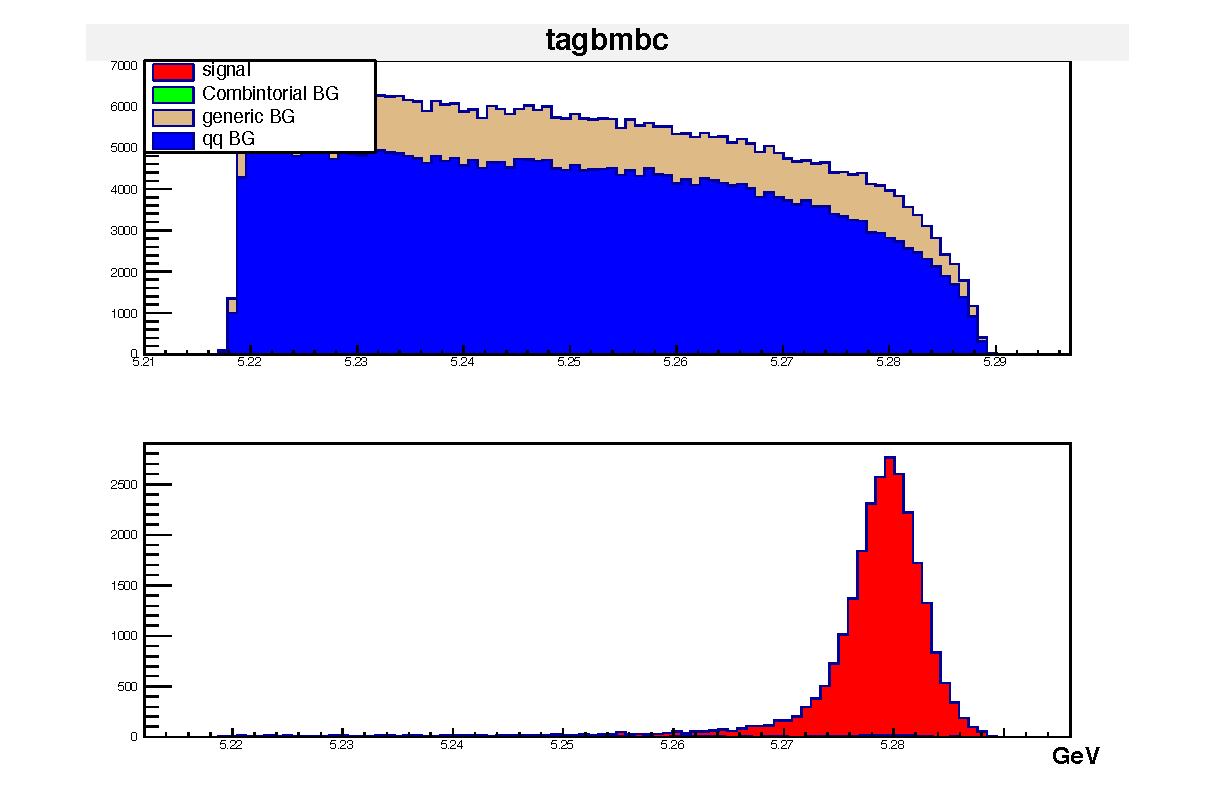
\includegraphics[width=0.45\textwidth]{eventselection_figure/tagbmbc_1025_1_b0ksh.eps}
		\label{ksmbc}
	}
	\caption{Tad-side $M_{bc}$ distribution for each mode. Red represent signal, green represent the combintorial background,  brown represent the generic background and blue represent continuum background.}
    	\label{fig:tagbmbc}	
\end{figure}


\begin{figure}[ht]
	\centering
	\subfigure[$K^{\pm}$ mode.]{
		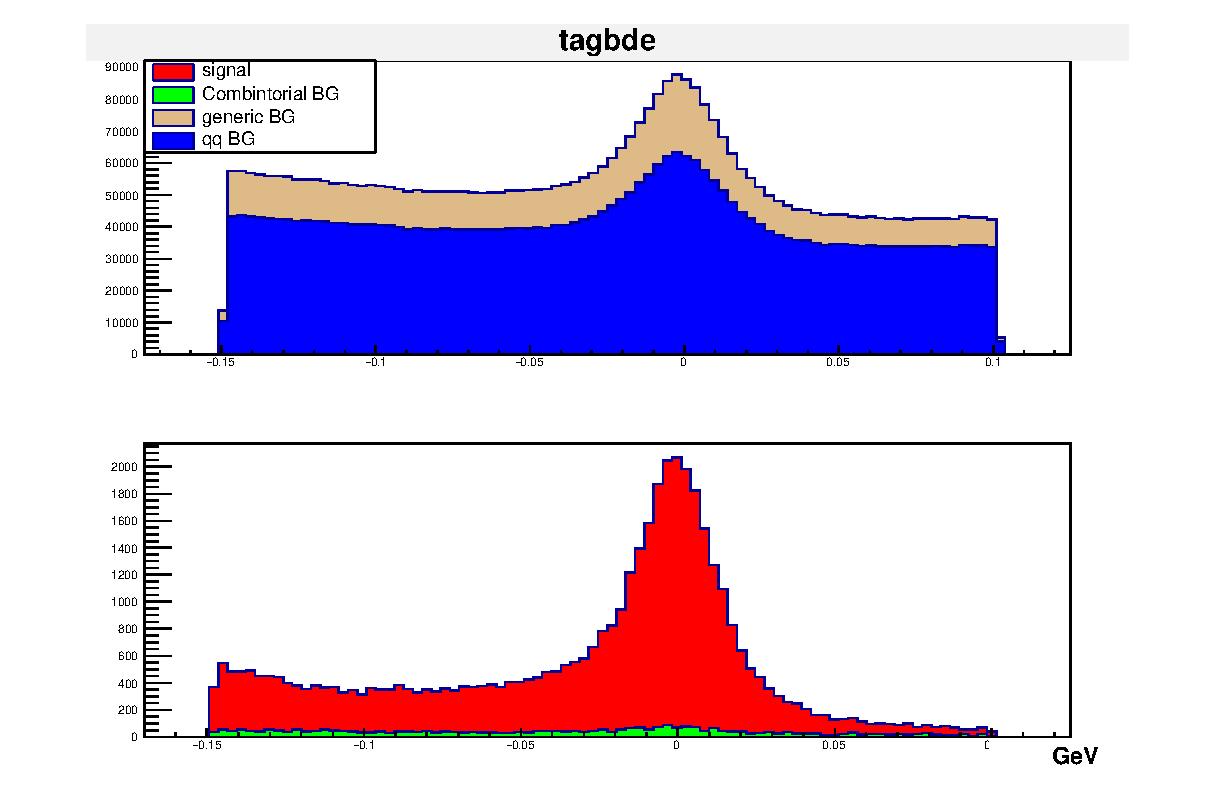
\includegraphics[width=0.45\textwidth]{eventselection_figure/tagbde_1025_1.eps}
		\label{kde}
	}
	\subfigure[$K^{*\pm} \rightarrow K^\pm \pi^0$ mode.]{
		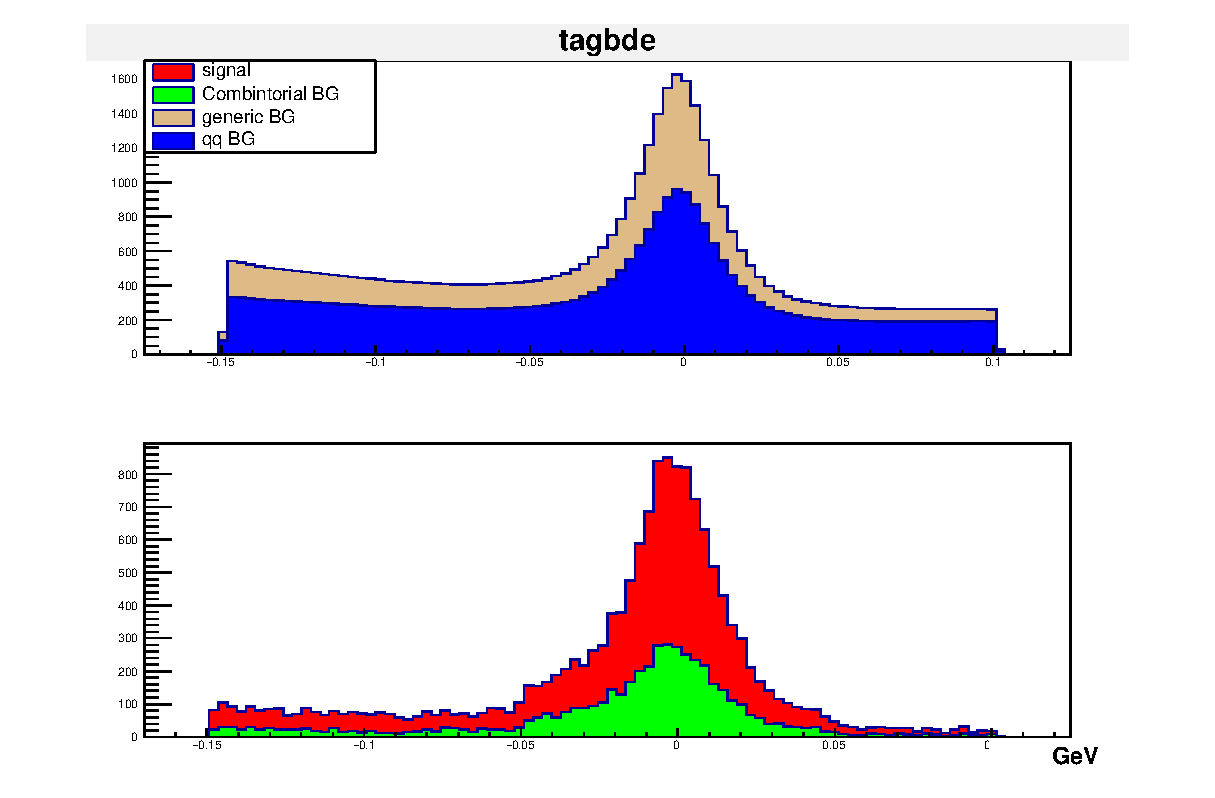
\includegraphics[width=0.45\textwidth]{eventselection_figure/tagbde_1025_1_kpi0.eps}
		\label{kpi0de}
	}
	\subfigure[$K^{*\pm} \rightarrow K_s \pi^\pm$ mode.]{
		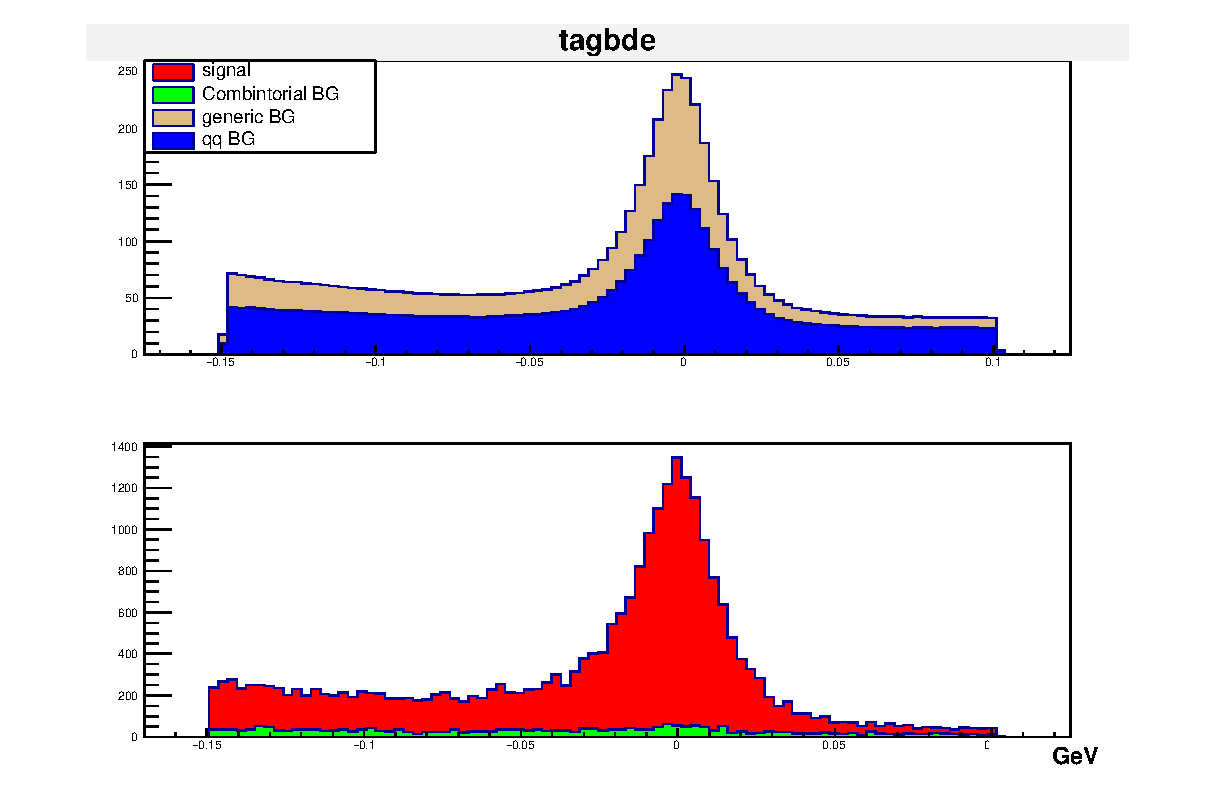
\includegraphics[width=0.45\textwidth]{eventselection_figure/tagbde_1025_1_kspi.eps}
		\label{kspide}
	}
    \subfigure[$K^{*0}$ mode.]{
		\includegraphics[width=0.45\textwidth]{eventselection_figure/tagbde_1025_1_b0kst.eps}
		\label{k0de}
	}
    \subfigure[$K_s$ mode.]{
		\includegraphics[width=0.45\textwidth]{eventselection_figure/tagbde_1025_1_b0ksh.eps}
		\label{ksde}
	}
	\caption{Tad-side $\Delta E$ distribution for each mode. Red represent signal, green represent the combinatorial background,  brown represent the generic background and blue represent continuum background.}
    	\label{fig:tagbde}	


    \end{figure}


    \begin{figure}[ht]
	\centering
	\subfigure[$K^{\pm}$ mode.]{
		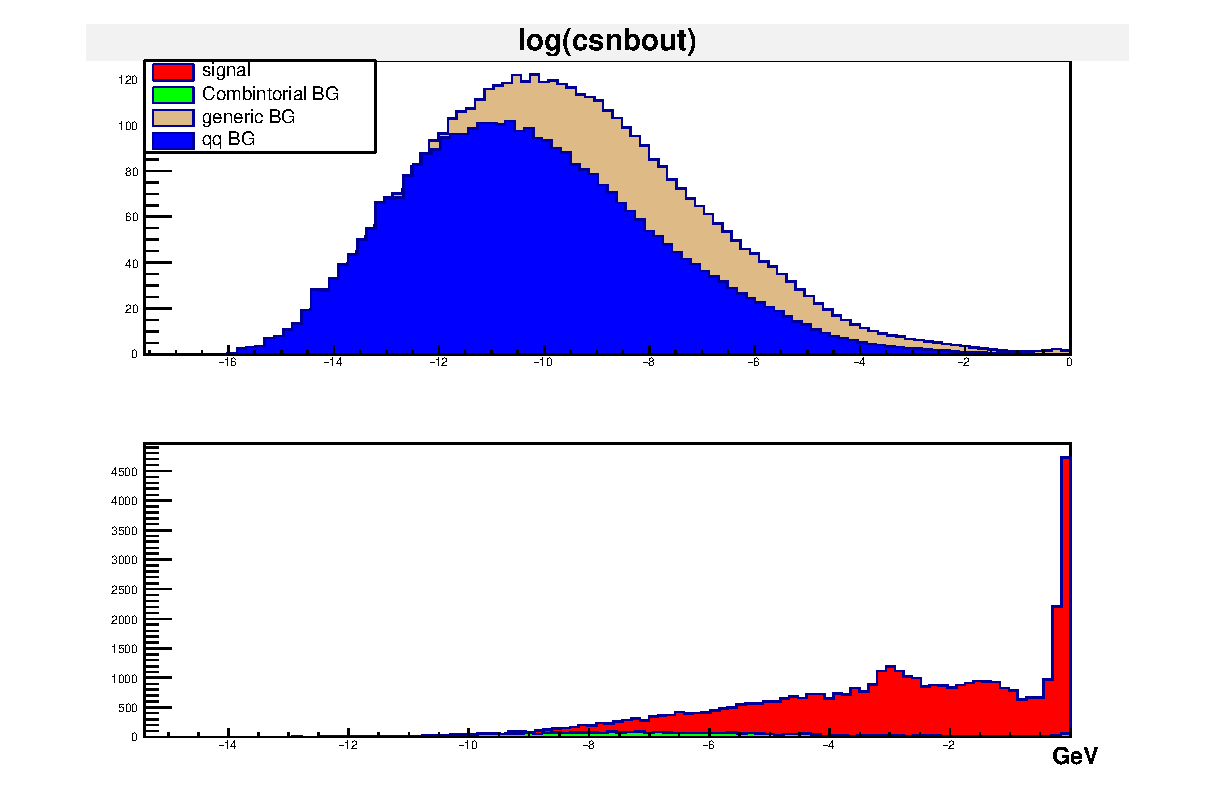
\includegraphics[width=0.45\textwidth]{eventselection_figure/log_csnbout__1025_1.eps}
		\label{knbout}
	}
	\subfigure[$K^{*\pm} \rightarrow K^\pm \pi^0$ mode.]{
		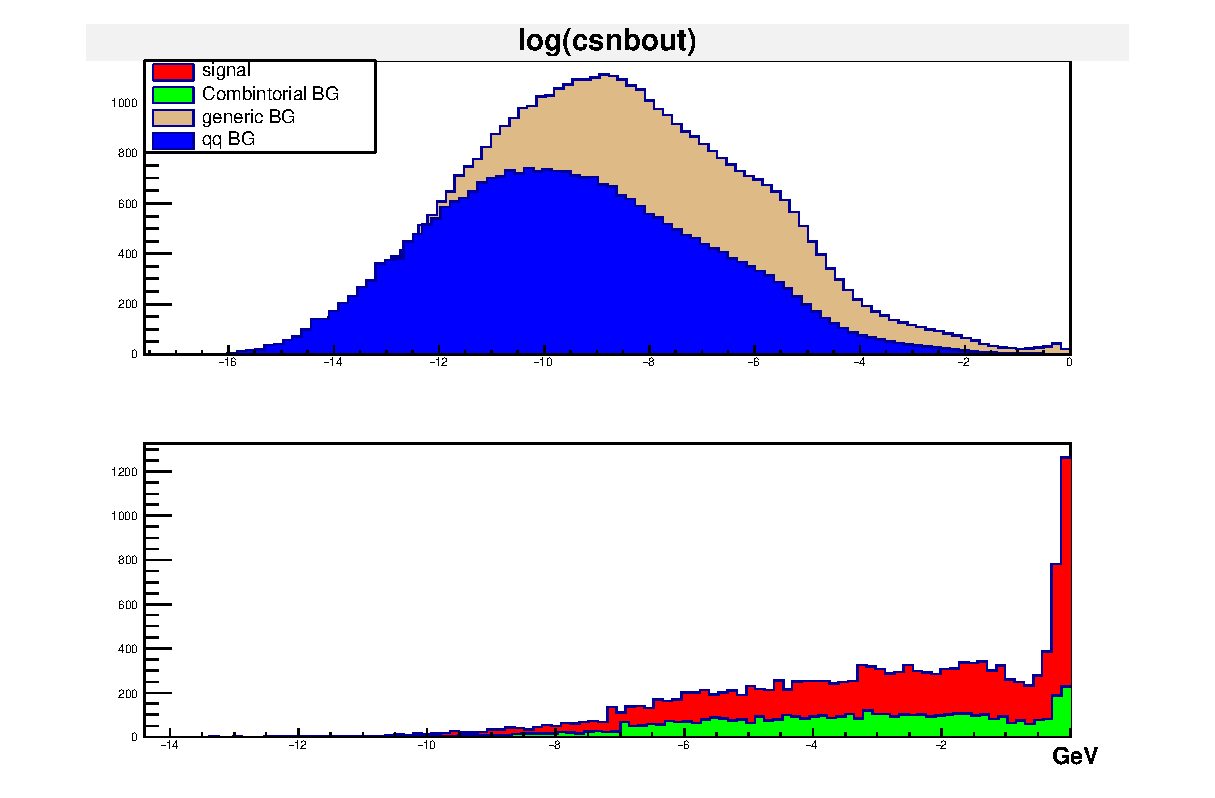
\includegraphics[width=0.45\textwidth]{eventselection_figure/log_csnbout__1025_1_kpi0.eps}
		\label{kpi0nbout}
	}
	\subfigure[$K^{*\pm} \rightarrow K_s \pi^\pm$ mode.]{
		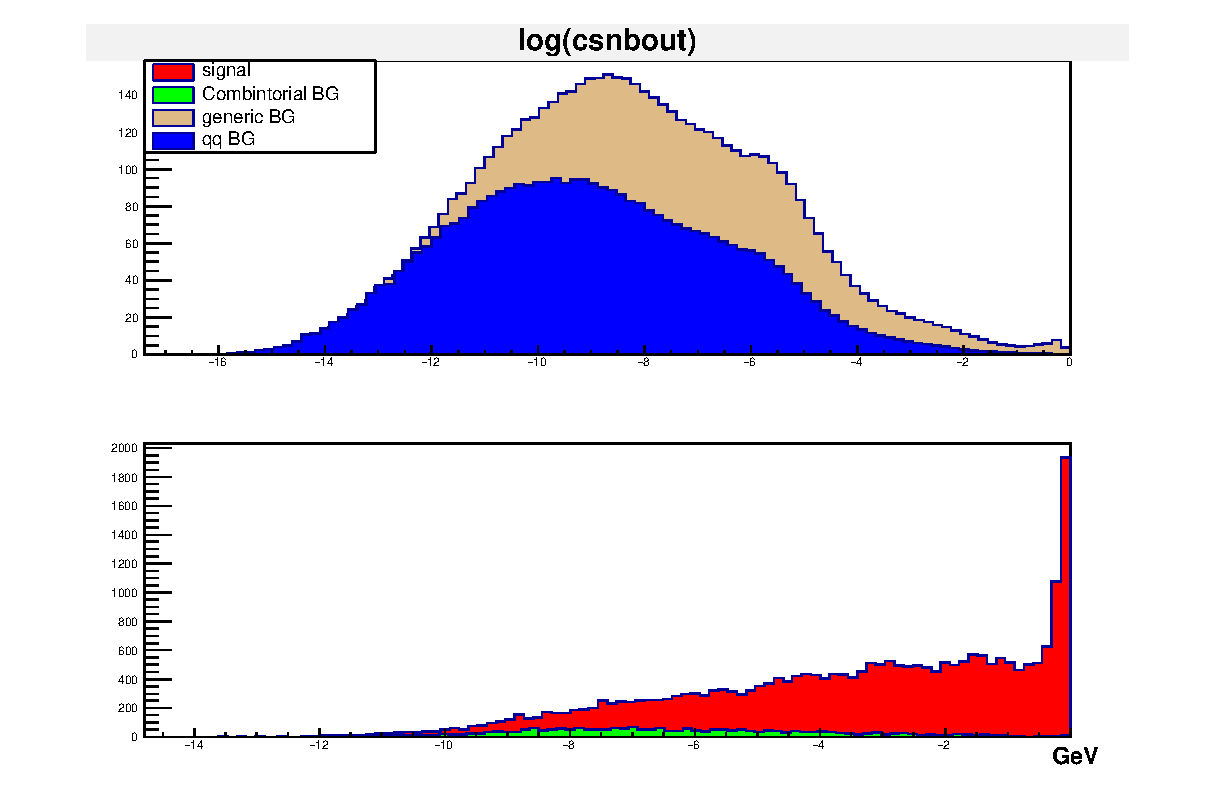
\includegraphics[width=0.45\textwidth]{eventselection_figure/log_csnbout__1025_1_kspi.eps}
		\label{kspinbout}
	}
    \subfigure[$K^{*0}$ mode.]{
		\includegraphics[width=0.45\textwidth]{eventselection_figure/log_csnbout__1025_1_b0kst.eps}
		\label{k0nbout}
	}
    \subfigure[$K_s$ mode.]{
		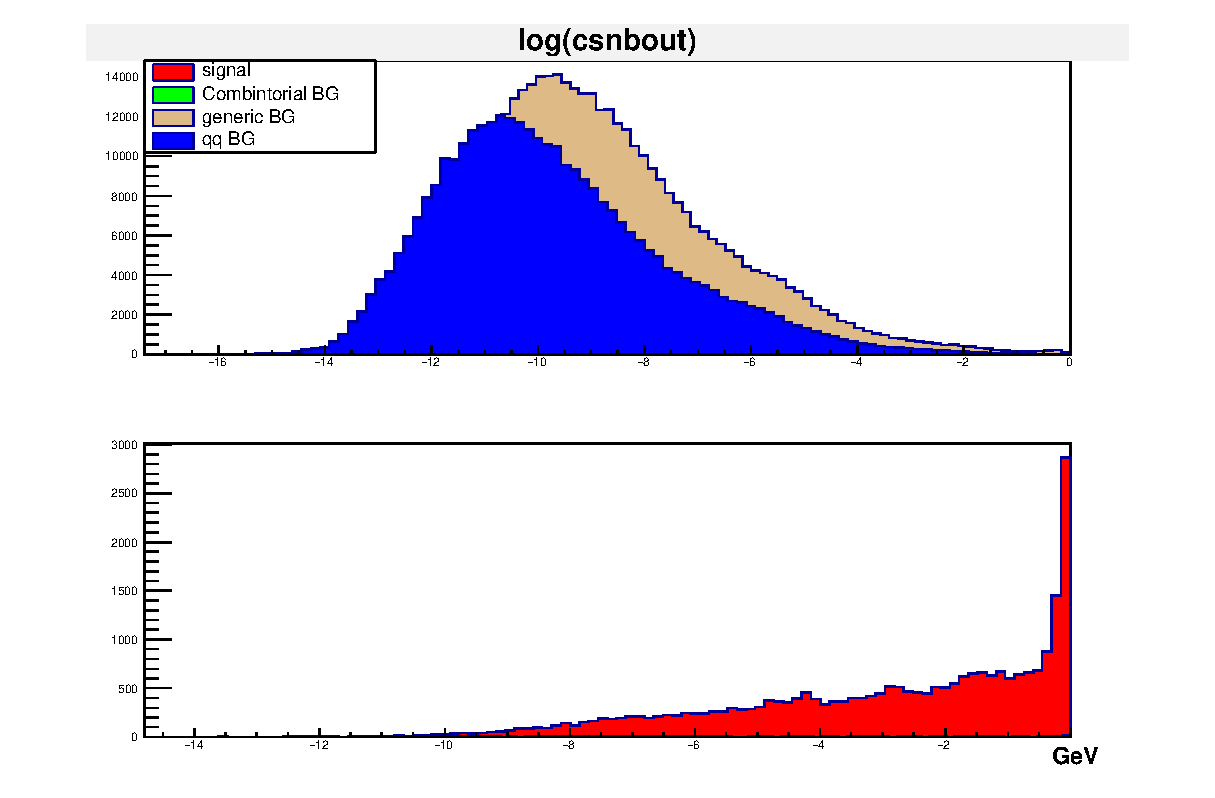
\includegraphics[width=0.45\textwidth]{eventselection_figure/log_csnbout__1025_1_b0ksh.eps}
		\label{ksnbout}
	}
	\caption{Tad-side NB output with continuum suppression $O_{tag}$ distribution for each mode. Red represent signal, green represent the combinatorial background,  brown represent the generic background and blue represent continuum background.}
    	\label{fig:nbout}	
\end{figure}

    \begin{figure}[ht]
	\centering
	\subfigure[$K^{\pm}$ mode.]{
		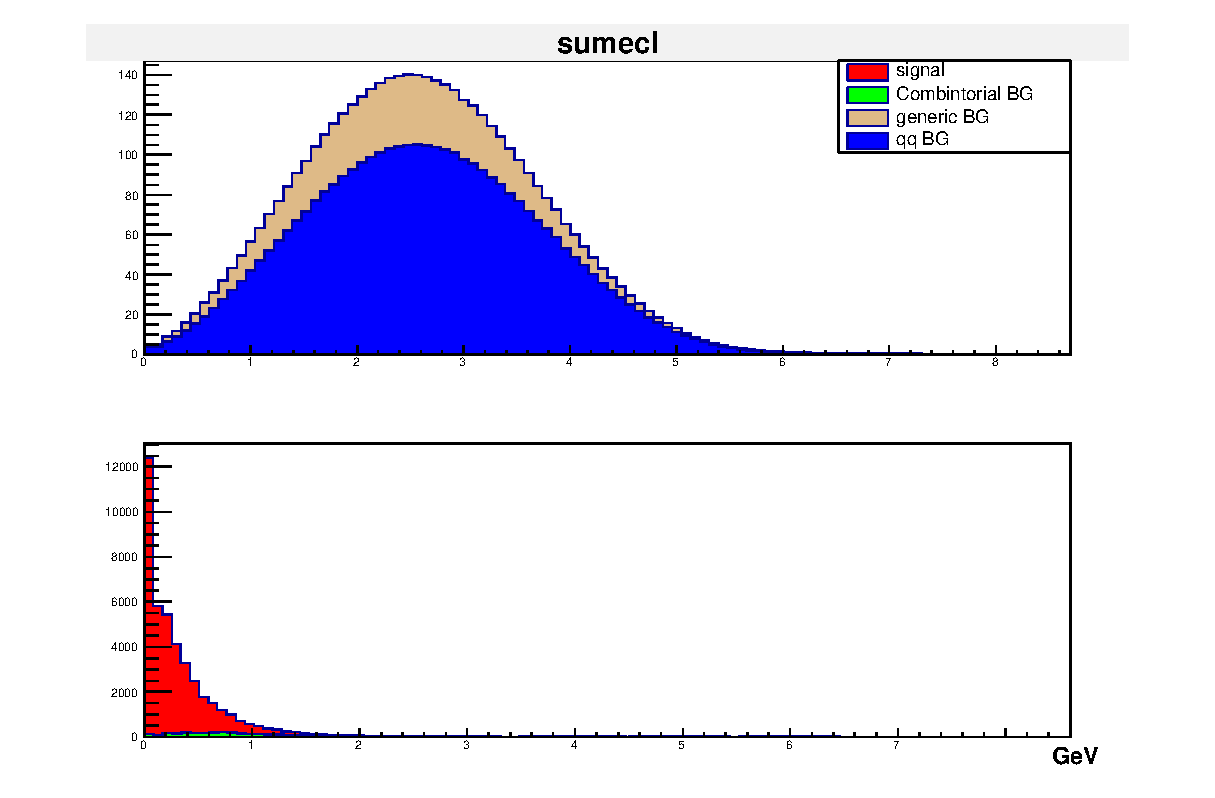
\includegraphics[width=0.45\textwidth]{eventselection_figure/sumecl_1025_1.eps}
		\label{ksumecl}
	}
	\subfigure[$K^{*\pm} \rightarrow K^\pm \pi^0$ mode.]{
		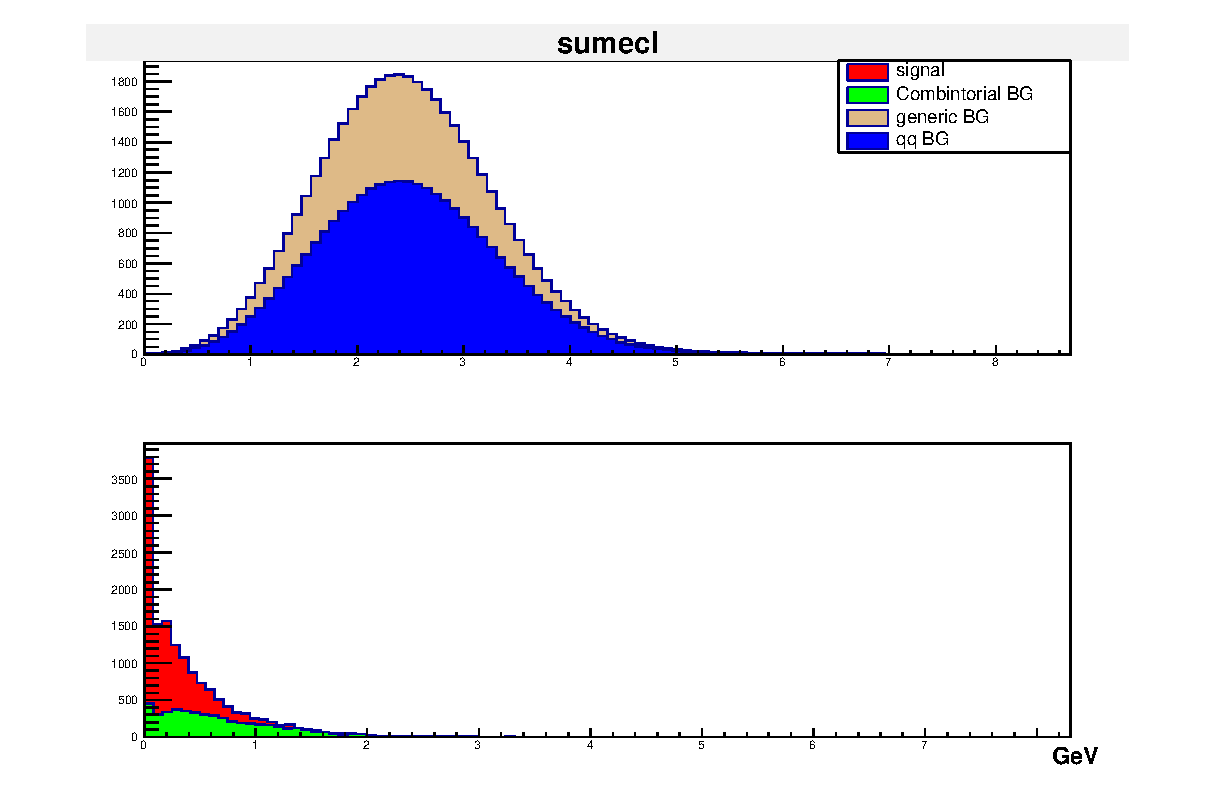
\includegraphics[width=0.45\textwidth]{eventselection_figure/sumecl_1025_1_kpi0.eps}
		\label{kpi0sumecl}
	}
	\subfigure[$K^{*\pm} \rightarrow K_s \pi^\pm$ mode.]{
		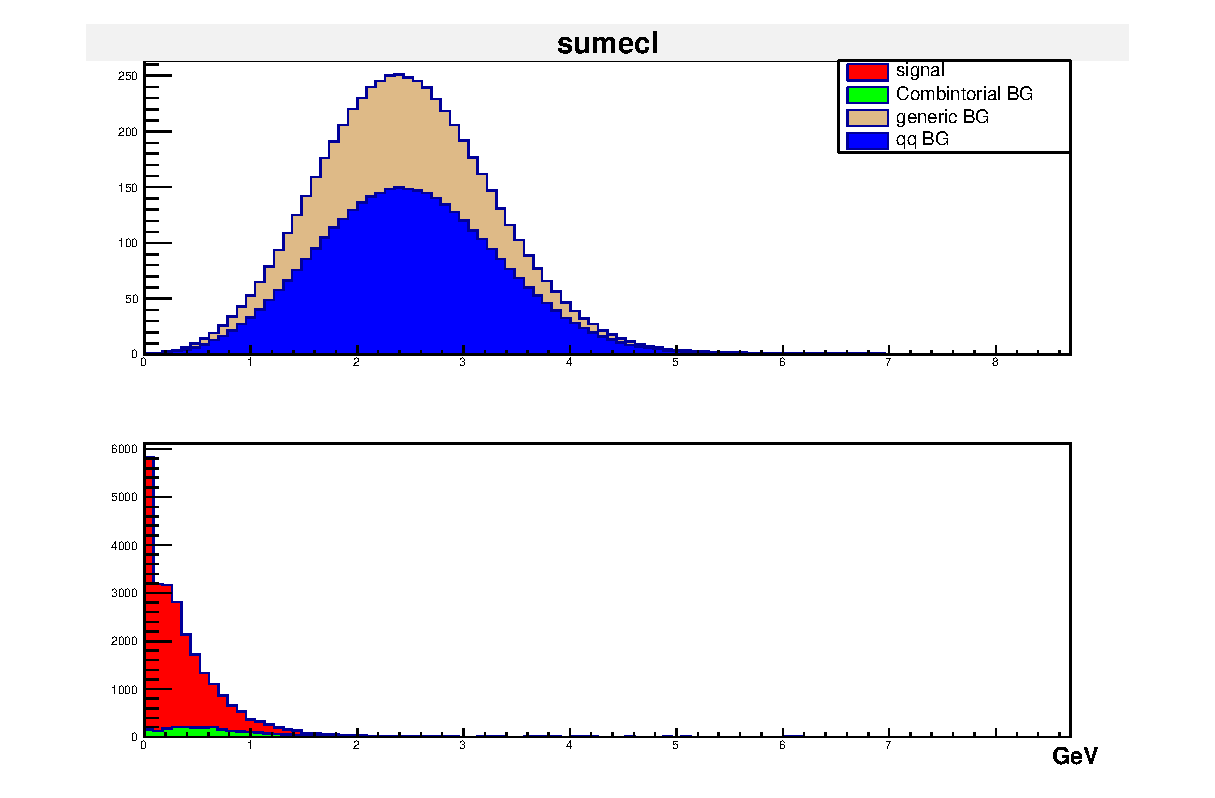
\includegraphics[width=0.45\textwidth]{eventselection_figure/sumecl_1025_1_kspi.eps}
		\label{kspisumecl}
	}
    \subfigure[$K^{*0}$ mode.]{
		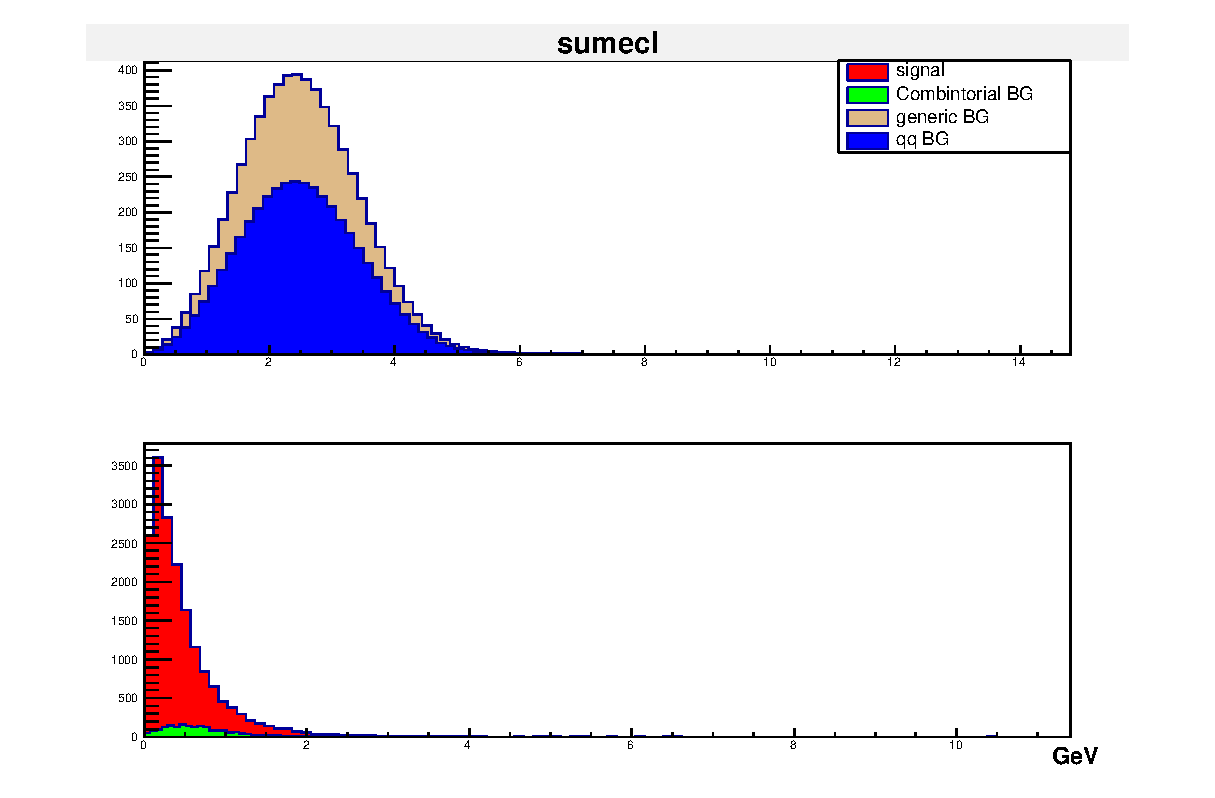
\includegraphics[width=0.45\textwidth]{eventselection_figure/sumecl_1025_1_b0kst.eps}
		\label{k0sumecl}
	}
    \subfigure[$K_s$ mode.]{
		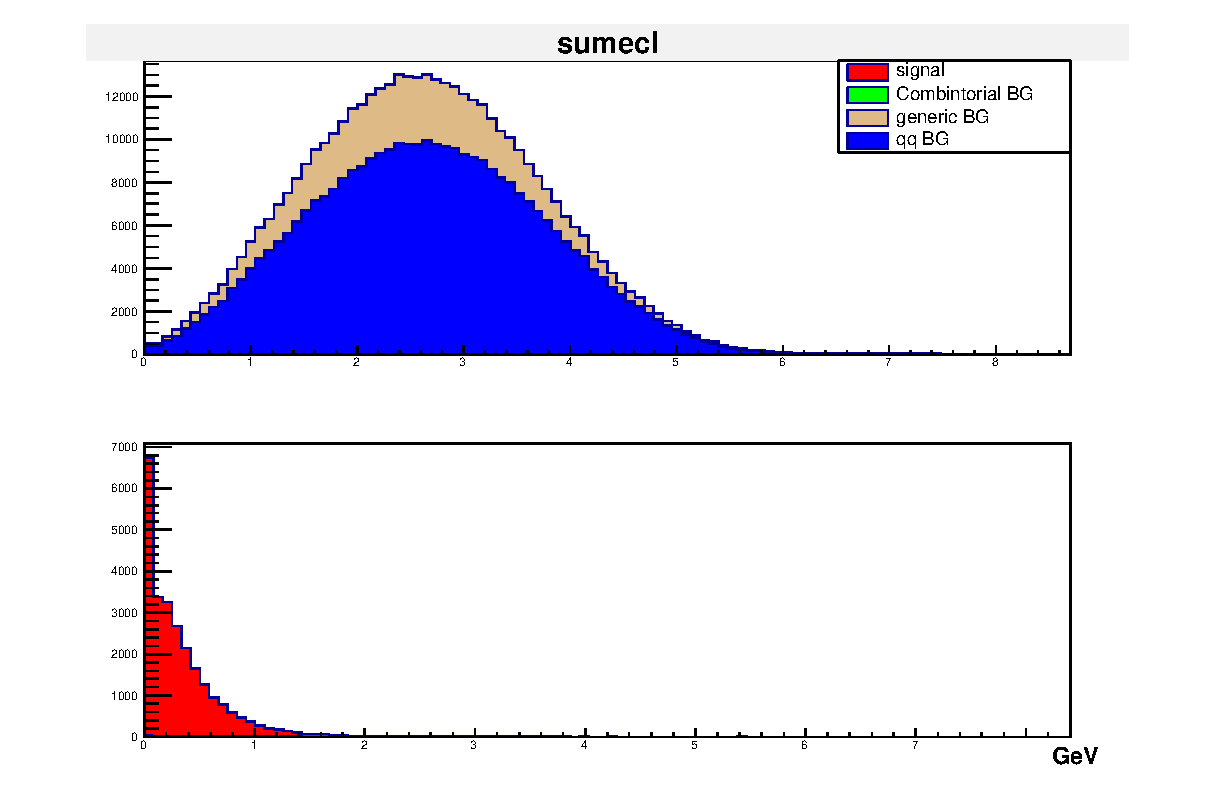
\includegraphics[width=0.45\textwidth]{eventselection_figure/sumecl_1025_1_b0ksh.eps}
		\label{kssumecl}
	}
\caption{Remaining energy $E_{ECL}$ distribution for each mode. Red represent signal, green represent the combinatorial background,  brown represent the generic background and blue represent continuum background.}
\label{fig:sumecl}	
\end{figure}
%%%%%%%%%%%%%%%%%%%%%%%%%%%%%%%%%%%%%%%%%%%%%%%%%%%%%%%%%%%%%%%%%%%%%%%%%%%%%%%%%%%%
\begin{table}[ht]
\small
\begin{center}
\begin{tabular}{ |p{2.2cm}||p{3.6cm}||p{2.8cm}||p{2.1cm}||p{1.3cm}|| }
\hline
 Cut					& Sig Efficiency$\times10^{-3}$  & generic BG$\times10^{4}$&qq BG$\times10^{4}$& com BG \\
\hline
\hline
  Fullrecon \& Track 		& $6.05\pm 0.03 $ 	& $ 10300\pm 1.01 $ 	&  $ 22900\pm1.51$	&7.30\%  \\ % &   $1.03 \times 10^{8}$&   $2.33 \times 10^{8}$ \\
 \hline
 $B_{\rm{tag}}M_{\rm{bc}} $  		& $5.96\pm 0.03$ 	& $ 6510\pm 0.81 $      & $ 14400\pm1.2 $	&4.50\%\\ %&   $3.77 \times 10^{7}$&   $8.93 \times 10^{7}$ \\
 \hline
 $ | B{\rm{tag}}\Delta E | $  		& $4.00 \pm 0.02$	& $ 3710\pm 0.61 $	& $  7430\pm0.86 $ 	&3.39\%\\ % &  $2.19 \times 10^{7}$ &   $4.70 \times 10^{7}$ \\
 \hline
 $E_{\rm{ecl}} $			& $3.96\pm 0.02$	& $ 969\pm 0.31$	& $ 1900\pm0.44 $ 	&2.88\%\\ % &  $5.86 \times 10^{6}$&   $1.22 \times 10^{7}$\\
 \hline
 n\_ track==0 				& $3.50\pm 0.02$	&$10.91\pm 0.03$	& $28.59\pm0.053$	&1.39\%\\ % &   $73524$&   $224138$ \\
 \hline		
$log(\rm{o_{tag}})$ 			& $3.45\pm 0.02$	&$6.35	\pm 0.03$	& $6.17 \pm0.024$	&1.12\% \\ %&   $1692$ &   $2555$\\
 \hline
\end{tabular}
\caption{$K^\pm$ mode: The efficiency drop and background level for each basic selection. The percentage of com BG means the fraction of the combinatorial background in signal MC. } \label{t:efficiency_k}

\end{center}
\end{table}

\begin{table}[ht]
 \small
\begin{center}
\begin{tabular}{ |p{2.2cm}||p{3.6cm}||p{2.8cm}||p{2.1cm}||p{1.3cm}|| }
 \hline
 Cut						& Sig Efficiency$\times10^{-3}$  & generic BG$\times10^{4}$&qq BG$\times10^{4}$& com BG \\
\hline
\hline
  Fullrecon \& Track 			& $1.37 \pm 0.01$ 	& $ 4496\pm0.67 $ 	&  $ 4849 \pm0.7$& 40.7\% \\ % &   $1.03 \times 10^{8}$&   $2.33 \times 10^{8}$ \\
 \hline
  $ M_{K^{* \pm}}  $  				& $1.29\pm 0.01$  	& $ 1560\pm0.40 $	& $ 370\pm0.19 $ & 32.5\%\\ % &   $5.95 \times 10^{7}$  &   $1.42 \times 10^{8}$\\
  \hline
 $B_{\rm{tag}}M_{\rm{bc}} $  			& $1.27\pm 0.01$ 	& $ 974\pm0.31$		& $ 229\pm0.15 $ &31.8\%\\ %&   $3.77 \times 10^{7}$&   $8.93 \times 10^{7}$ \\
 \hline
 $ | B{\rm{tag}}\Delta E | $  			& $1.00\pm 0.01$	& $ 586 \pm0.24$	& $ 132\pm0.12 $ &33.2\%\\ % &  $2.19 \times 10^{7}$ &   $4.70 \times 10^{7}$ \\
 \hline
 $E_{\rm{ecl}} $				& $0.999\pm 0.01 $	& $ 173\pm0.13$		& $ 38\pm0.06 $ &32.9\%\\ % &  $5.86 \times 10^{6}$&   $1.22 \times 10^{7}$\\
 \hline
 n\_ track==0 					& $0.977\pm 0.01 $	& $0.34\pm0.006$ 	& $2.3\pm0.02$  &32.5\%\\ % &   $73524$&   $224138$ \\
 \hline		
$log(\rm{o_{tag}})$ 				& $0.957\pm 0.01 $	& $0.18\pm0.004$	& $0.54\pm0.007$ &32.7\% \\ %&   $1692$ &   $2555$\\
 \hline
\end{tabular}
\caption{$K^{*\pm} \rightarrow K^+ \pi^0$ mode: The efficiency drop and background level for each basic selection. The percentage of com BG means the fraction of the combinatorial background in signal MC. } \label{t:efficiency_kpi0}
\end{center}
\end{table}
%%%%%%%%%%%%%%%%%%%%%%%%%%%%%%%%%%%%%%%%%%%%%%%%%%%%%%%%%%%%%%%%%%%%%%%%%%%%%%%%%%%%%%
\begin{table}[ht]
 \small
\begin{center}
\begin{tabular}{ |p{2.2cm}||p{3.6cm}||p{2.8cm}||p{2.1cm}||p{1.3cm}|| }
 \hline
 Cut& Sig Efficiency$\times10^{-3}$  & generic BG$\times10^{4}$&qq BG$\times10^{4}$& com BG \\
\hline
\hline
  Fullrecon \& Track 			& $2.981 \pm 0.02$ 	& $ 278 \pm 0.17$ 	&  $ 432 \pm 0.21$& 9.8\% \\ % &   $1.03 \times 10^{8}$&   $2.33 \times 10^{8}$ \\
 \hline
  $  M_{K^{* \pm}}  $  				& $2.979 \pm 0.02$  	& $ 228 \pm 0.15$	& $ 370 \pm 0.19$ & 9.7\%\\ % &   $5.95 \times 10^{7}$  &   $1.42 \times 10^{8}$\\
  \hline
 $B_{\rm{tag}}M_{\rm{bc}} $  			& $2.94 \pm 0.02$ 	& $ 142 \pm 0.11$	 & $ 229 \pm 0.15$ &6.5\%\\ %&   $3.77 \times 10^{7}$&   $8.93 \times 10^{7}$ \\
 \hline
 $ | B{\rm{tag}}\Delta E | $  			& $2.09 \pm 0.02$	& $88.32\pm 0.09$	& $132\pm 0.12$ &4.3\%\\ % &  $2.19 \times 10^{7}$ &   $4.70 \times 10^{7}$ \\
 \hline
 $E_{\rm{ecl}} $				& $2.07 \pm 0.02$	& $26.68\pm 0.05$	& $37.5\pm 0.06$ &4.2\%\\ % &  $5.86 \times 10^{6}$&   $1.22 \times 10^{7}$\\
 \hline
 n\_ track==0 					& $1.98 \pm 0.02$	&$0.879\pm 0.01 $	& $2.35\pm 0.015$  &3.3\%\\ % &   $73524$&   $224138$ \\
 \hline		
$log(\rm{o_{tag}})$ 				& $1.91 \pm 0.02$	&$0.490\pm 0.007$ 	& $0.54\pm 0.007$ &2.6\% \\ %&   $1692$ &   $2555$\\
 \hline
\end{tabular}
\caption{$K^{*\pm} \rightarrow K_s \pi^\pm$ mode: The efficiency drop and background level for each basic selection. The percentage of com BG means the fraction of the combinatorial background in signal MC. } \label{t:efficiency_kspi}
\end{center}
\end{table}

\begin{table}[ht]
 \small
\begin{center}
\begin{tabular}{ |p{2.2cm}||p{3.6cm}||p{2.8cm}||p{2.1cm}||p{1.3cm}|| }
 \hline
 Cut& Sig Efficiency$\times10^{-3}$  & generic BG$\times10^{4}$&qq BG$\times10^{4}$& com BG \\
\hline
\hline
  Fullrecon \& Track\&$M_{K*0} $	& $(2.47\pm 0.02)$ 	&$1558\pm  0.395$&$2771\pm 0.526$&9.88\% \\ % &   $1.03 \times 10^{8}$&   $2.33 \times 10^{8}$ \\
 \hline
 $B_{\rm{tag}}M_{\rm{bc}}$  			& $(2.44\pm 0.02)$ 	&$972 \pm 0.312$&$1716 \pm 0.414$&6.59\%\\ %&   $3.77 \times 10^{7}$&   $8.93 \times 10^{7}$ \\
 \hline
 $ | B{\rm{tag}}\Delta E |$  			& $(1.79\pm 0.02)$	&$585 \pm 0.242$&$953 \pm0.309$	&4.00\%\\ % &  $2.19 \times 10^{7}$ &   $4.70 \times 10^{7}$ \\
 \hline
 $E_{\rm{ecl}}$					& $(1.78\pm 0.02$	&$173  \pm 0.132$&$270\pm0.164$	&3.94\%\\ % &  $5.86 \times 10^{6}$&   $1.22 \times 10^{7}$\\
 \hline
 n\_ track					& $(1.73 \pm 0.02)$	&$13.3\pm 0.04$	&$22.9\pm0.048$	&0.79\%\\ % &   $73524$&   $224138$ \\
 \hline		
$log(\rm{o_{tag}})$ 				& $(1.70 \pm0.01)$	&$7.64\pm0.03$	&$4.98\pm0.022$	&0.72\% \\ %&   $1692$ &   $2555$\\
 \hline
\end{tabular}
\caption{$K^{*0}$ mode: The efficiency drop and background level for each basic selection. The percentage of com BG means the fraction of the combintorial background in signal MC. } \label{t:efficiency_k0}
\end{center}
\end{table}
%%%%%%%%%%%%%%%%%%%%%%%%%%%%%%%%%%%%%%%%%%%%%%%%%%%%%%%%%%%%%%%%%%
\begin{table}[ht]
 \small
\begin{center}
\begin{tabular}{ |p{2.2cm}||p{3.6cm}||p{2.8cm}||p{2.1cm}||p{1.3cm}|| }
 \hline
 Cut& Sig Efficiency$\times10^{-3}$  & generic BG$\times10^{4}$&qq BG$\times10^{4}$& com BG \\
\hline
\hline
  Fullrecon \& Track\&$M_{K*0} $	& $(3.53\pm 0.02)$ &$601\pm 0.245$&$1210\pm 3479$	&2.77\% \\ % &   $1.03 \times 10^{8}$&   $2.33 \times 10^{8}$ \\
 \hline
 $B_{\rm{tag}}M_{\rm{bc}}$  		& $(3.49\pm 0.02)$ &$383 \pm 0.196$&$761 \pm 0.275$	&1.70\%\\ %&   $3.77 \times 10^{7}$&   $8.93 \times 10^{7}$ \\
 \hline
 $ | B{\rm{tag}}\Delta E |$  		& $(2.56\pm 0.02)$	&$223 \pm 0.149$&$401 \pm0.200$	&1.23\%\\ % &  $2.19 \times 10^{7}$ &   $4.70 \times 10^{7}$ \\
 \hline
 $E_{\rm{ecl}}$				& $(2.52 \pm 0.02$	&$57\pm0.076$&$97\pm0.099$	&1.19\%\\ % &  $5.86 \times 10^{6}$&   $1.22 \times 10^{7}$\\
 \hline
 n\_ track					& $(2.40 \pm 0.02)$	&$0.95\pm0.01$&$2.69\pm0.016$	&0.79\%\\ % &   $73524$&   $224138$ \\
 \hline		
$log(\rm{o_{tag}})$ 				& $(2.33\pm0.02)$	&$0.53\pm0.007$&$0.56\pm0.008$	&0.72\% \\ %&   $1692$ &   $2555$\\
 \hline
\end{tabular}
\caption{$K_s$ mode: The efficiency drop and background level for each basic selection. The percentage of com BG means the fraction of the combinatorial background in signal MC. } \label{t:efficiency_ks}\end{center}
\end{table}
%%%%%%%%%%%%%%%%%%%%%%%%%%%%%%%%%%%%%%%%%%%%%%%%%%%%%%%%%%%%%%%%%%%%%%%%%%%%%%%%%%%%%
